\chapter{Creación de un espectáculo de \emph{video mapping}}

\section{Introducción}
En la creación de un espectáculo de \emph{video mapping} se identifican tres etapas que son el modelado de la escena, la producción del espectáculo y la proyección del mismo.

En el modelado de la escena se obtiene una representación virtual y abstracta de los objetos reales sobre los que se proyectará. Este modelo será la base para trabajar en posteriores etapas y sobre el cuál se diseñará el espectáculo.

En la siguiente etapa se realiza la producción del espectáculo que consiste en aplicar distintos efectos visuales sobre los objetos modelados y orquestar la ejecución de los mismos. En esta etapa también se diseña y produce la musicalización que será utilizada durante todo el espectáculo.
%Orquestar no aplica para toques en vivo, hay que explicar este caso también y reescribir.%

Es en la proyección del espectáculo en donde se puede contemplar el resultado de los distintos efectos visuales proyectados sobre las superficies acompañados por efectos de sonido.
Para lograr la correspondencia en la proyección de los objetos del modelo con las superficies se debe calibrar la proyección. Esta correspondencia se logra modificando el modelo de la escena, ajustando la posición y orientación de los proyectores, y ajustando los parámetros intrínsecos$^\dagger$ de la proyección.
%Esta etapa no es necesariamente una proyeccion final sino que se puede simular%

Cada una de estas etapas se puede abordar con un enfoque bidimensional o tridimensional.
Con un enfoque bidimensional el modelo de la escena es una proyección en perspectiva de los objetos a proyectar, por ejemplo, una fotografía. Con un enfoque tridimensional el modelo se mantiene independiente de un punto de vista, representándose con un conjunto de objetos virtuales tridimensionales.

%explicacion de pie de diagrama:redactarlo mejor, El modelo generado en 2d depende del punto de vista del proyector y puede no parecerse a la realidad. El modelo generado 3d se asimila a la realidad y luego con la cámara virtual ajusto el punto de vista del proyector.

\begin{figure}[H]
  \centering
    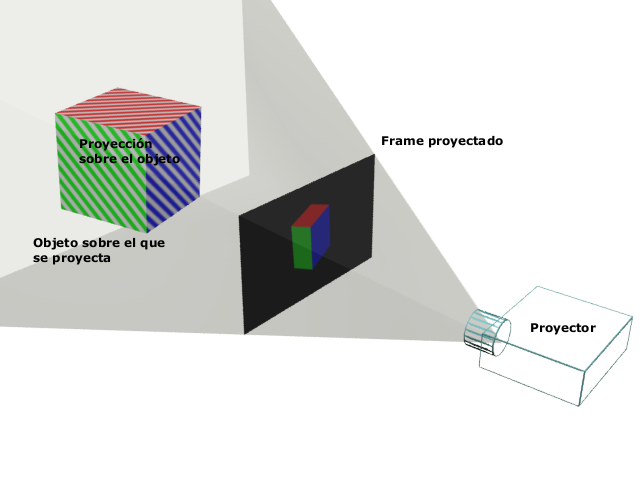
\includegraphics[width=0.7\textwidth]{./Cap2_videomapping/proy2dvs3d}
  \caption{Esquema de proyección.}
  \label{fig:proy2dvs3d}
\end{figure}

\section{Enfoque bidimensional}
\subsection{Modelo}
Un modelo bidimensional refleja lo que vería un observador desde un punto de vista fijo.
%si se quieren agregar hay en el SVN imagenes de proyeccion perspectiva y paralela  VER
Técnicamente es el resultado de una proyección en perspectiva \cite{LibroCompGrafica} sobre un plano de vista de los elementos de la superficie a modelar.

Este punto de vista debe ser considerado al posicionar y orientar el proyector que reproducirá el espectáculo.
La posición, orientación y campo de vista del proyector definirán además la sección de superficie sobre la que se proyectará.
En caso de utilizar más de un proyector cada uno de estos será posicionado en un lugar diferente y por lo tanto será necesario un modelo por cada uno de ellos.

\begin{figure}[H]
  \centering
    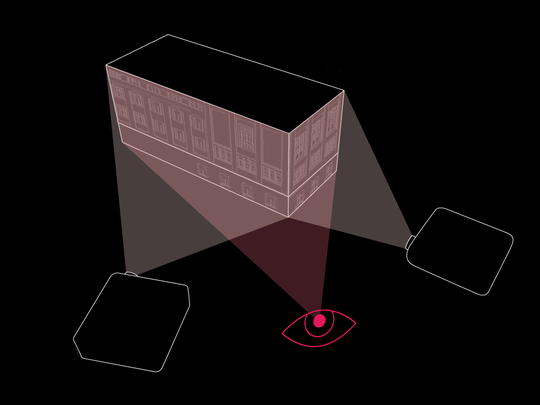
\includegraphics[width=0.7\textwidth]{./Cap2_videomapping/diagrama-2proyectores}
  \caption{Proyectores y sus puntos de vista.}%referenciar imagen%
  \label{fig:diagrama-2proyectores}
\end{figure}

Son ejemplos de modelos una fotografía, un plano arquitectónico de una fachada o figuras geométricas bidimensionales que representan las secciones de las superficies. En algunos casos estos se combinan para obtener como resultado un único modelo.
\begin{itemize}
  \item Una fotografía. Ubicando la cámara de forma que su punto de vista y el del proyector coincidan minimizará los ajustes necesarios en la etapa de calibración.%extender y que no quede tan en el aire lo de ajustes de calibracion%
  \item Un plano arquitectónico contiene información exacta de las medidas de la superficie que representa en una escala dada. Generalmente utiliza el método de proyecciones paralelas \cite{LibroCompGrafica} sobre un plano de proyección. Para utilizar el plano arquitectónico como modelo se debe transformar de forma que coincida con la proyección en perspectiva desde el punto vista que estará ubicado el proyector.
  \item Las figuras geométricas modelan sectores de la superficie donde se proyectará. Un método para generar las figuras geométricas consiste en utilizar un proyector y herramientas de software que permiten delinear el contorno de las secciones de la superficie en tiempo real. Se observa el resultado de cada figura generada proyectada sobre la superficie ajustando el modelo en el momento de la construcción.%%%figuras geometricas queda muy abstracto, hay que llevarlo mas al tema de representacion digital de quads%%%
\begin{figure}[H]
  \centering
    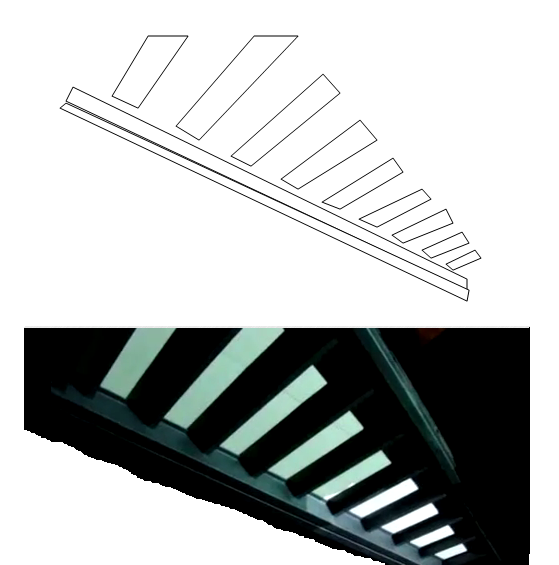
\includegraphics[width=0.7\textwidth]{./Cap2_videomapping/RepresentacionconfigurasGeometricas}
  \caption{Representación con figuras geométricas.}
  \label{fig:RepresentacionconfigurasGeometricas}
\end{figure}

Al usar el proyector para obtener el modelo queda incorporada la perspectiva del mismo y si no se modifica su posición y orientación no sería necesaria otra calibración.
Otra opción es dibujar las figuras con una fotografía o plano de fondo. En este caso la construcción de las figuras geométricas se realiza delineando el contorno de la superficie en la fotografía o plano.
Una forma automática de generar el modelo es utilizando técnicas de visión por computadora$^\dagger$, por ejemplo, en base a algoritmos de reconocimiento de aristas \cite{ArticuloAutom2dmodel}.
\end{itemize}

\subsection{Producción del espectáculo}
La producción del espectáculo en dos dimensiones consiste en definir efectos visuales sobre regiones de un espacio bidimensional discreto$^\dagger$ representadas en el modelo de la escena. Este espacio bidimensional discreto se representa con coordenadas de pantalla que identifican cada uno de los píxeles$^\dagger$ del área de trabajo. Los efectos visuales se logran realizando cualquier animación computacional que genere una salida gráfica como pueden ser videos e imágenes.
En esta etapa, además de definir los efectos, se planifica en qué momento se mostrarán cada uno de ellos, pudiendo sincronizarse con la música que forma parte del espectáculo.
%Mencionar caso de espectaculos en vivo%

En computación gráfica se utilizan texturas para proyectar videos e imágenes sobre regiones del área de trabajo. Las texturas son mapas de bits$^\dagger$ utilizados para cubrir la superficie de un objeto virtual. Estos mapas de bits pueden ser generados a partir de imágenes, videos, o incluso dinámicamente mediante algoritmos permitiendo así crear efectos visuales como, por ejemplo, la transición de un color a otro.
Cuando se utilizan videos estos pueden ser generados teniendo en cuenta la superficie donde se está proyectando y el punto de vista desde donde se contemplará el espectáculo. Esto es particularmente importante cuando el contenido a mostrar pretende crear una ilusión tridimensional, pues la perspectiva debe coincidir con la de los espectadores.%ampliar o explicar mejor%
\begin{figure}[H]
  \centering
    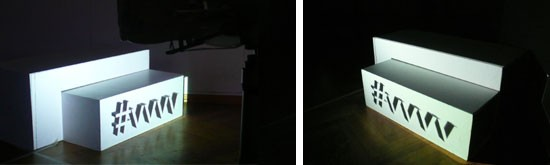
\includegraphics[width=0.7\textwidth]{./Cap2_videomapping/3dillusion}
  \caption{Izq. Ilusión 3D lograda. Der. No se logra la ilusión.}%ref%
  \label{fig:3dillusion}
\end{figure}

En este contexto se habla de mapeo, no como la salida a través de un equipo proyector, sino como la operación que logra una correspondencia entre una textura y una figura geométrica que no necesariamente coinciden en tamaño y forma. Para esto se definen coordenadas de textura en cada vértice de la figura geométrica que referencian distintas ubicaciones dentro de la misma.
Las coordenadas de las texturas tienen dos componentes: una horizontal y una vertical llamadas U y V. Si el valor de estas componentes se normaliza entre 0 y 1 entonces la esquina superior izquierda de la textura se corresponderá con la coordenada (0,0), la superior derecha con (1,0), la inferior izquierda con (0,1) y la inferior derecha con (1,1).
%agregar referencia a correspondencia de textura en un objeto, ver para imagen http://en.wikipedia.org/wiki/UV_mapping
Los vértices de una figura geométrica se asocian con coordenadas UV que definen el punto de la textura que se corresponde sobre el vértice. Mediante interpolación se logra mapear toda la textura a la figura geométrica.
Si bien es posible mapear una textura a cualquier figura geométrica, esta correspondencia es más directa utilizando un cuadrilátero ya que a cada uno de los vértices se lo hace corresponder con una esquina de la textura. A su vez el cuadrilátero es la figura básica en las aplicaciones\footnote{Las aplicaciones relevadas utilizan el cuadrilátero como figura básica. Ver apéndice: Aplicaciones relevadas.} de \emph{video mapping}.
Estos cuadriláteros se utilizan como piezas constructoras del espectáculo, cubriendo sectores del modelo sobre los cuales luego se aplican las texturas permitiendo crear los distintos efectos visuales.

\subsection{Calibración}
La calibración se utiliza para ajustar el modelo con la superficie que representa. Inicialmente se fija la posición y orientación del proyector y luego, con ayuda de herramientas de software, se aplica la transformación geométrica homografía\footnote{Ver sección: Obtención de geometría} a la proyección resultante, para lograr la correspondencia.
En caso de haber modificaciones en la posición y orientación del proyector la calibración deberá realizase nuevamente. %reescribir esta oración%

Los ajustes necesarios varían dependiendo del método utilizado para obtener el modelo. En caso de utilizar una fotografía, el proyector deberá ser ubicado de forma tal que el punto de vista de la cámara con la que se tomó coincida con el del proyector y así lograr la coincidencia del centro de proyección. Igualmente son necesarios ajustes ya que los lentes de la cámara y el proyector no necesariamente coinciden en el ángulo de visión \cite{LibroCompGrafica2}\cite{LibroPhotographicOptics}. Con el método de generación de figuras geométricas, en el que se modelan las secciones de la superficie a mapear utilizando el mismo proyector, los ajustes se reducen a lograr la misma posición y orientación que tenía el proyector al momento de la captura de secciones, ya que las deformaciones relacionadas a los parámetros intrínsecos fueron implícitamente consideradas durante el proceso de captura.

\section{Enfoque tridimensional}
\subsection{Modelo}
Para el modelado tridimensional se pueden utilizar representaciones de cuerpos y superficies tridimensionales representadas por mallas$^\dagger$ de polígonos \cite{Mesh_building}, comúnmente utilizadas en disciplinas como cartografía, visión computacional y computación gráfica. A diferencia de un modelo bidimensional, éste no depende de un punto de vista, lo que permite al diseñador visualizar la escena desde diferentes ángulos. Las entidades que conforman la malla son vértices, aristas, caras y atributos numéricos que representan la posición y normales de los vértices, coordenadas de textura y colores. La topología de la malla puede variar, por ejemplo, los polígonos que la componen pueden tener distinta cantidad de vértices.

\begin{minipage}{0.35\textwidth}
\begin{flushleft} \large
\begin{figure}[H]
  \centering
    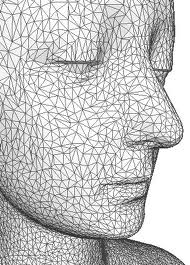
\includegraphics[width=0.7\textwidth]{./Cap2_videomapping/EjemploMallaTriangular}
  \caption{Mallas triangulares.}%ref%
  \label{fig:mallas1}
\end{figure}
\end{flushleft}
\end{minipage}
\begin{minipage}{0.45\textwidth}
\begin{flushright} \large
\begin{figure}[H]
  \centering
    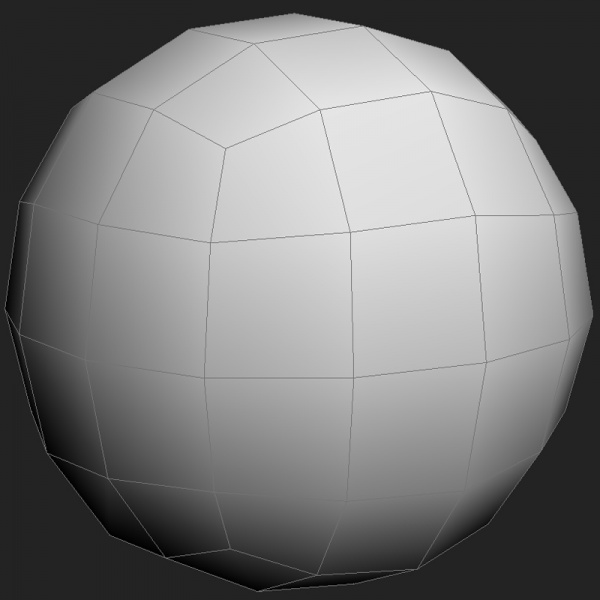
\includegraphics[width=0.75\textwidth]{./Cap2_videomapping/EjemploMalla4Vertices}
  \caption{Mallas de cuadriláteros.}%ref%
  \label{fig:mallas2}
\end{figure}

\end{flushright}
\end{minipage}

Es muy común que las mallas contengan información redundante, para lo que existen técnicas como la de \emph{remeshing} que mediante la utilización de algoritmos específicos reducen la cantidad de vértices de la malla sin perder la representatividad de la superficie.
%si se quiere se pone esta referencia:Survey of Polygonal Surface Simplification Algorithms Paul S. Heckbert and Michael Garland doc/papers/Mesh_building/Survey of Polygonal Surface Simplification Algorithms.pdf

Los modelos tridimensionales se generan utilizando distintas técnicas:
\begin{itemize}
  \item Modelado utilizando polígonos: a partir de mallas que representan figuras primitivas se podrán construir nuevas mallas, por ejemplo aplicando operaciones de unión o resta.
  %Que es union y resta?, explicar esto o algo mas general, union y resta son solo dos ejemplos y no los mas representativos%
  También se aplican transformaciones que modifican las aristas, vértices o caras, aproximando el resultado a la superficie que se desea modelar.
  \item  Modelado utilizando curvas: a partir de una jaula creada por curvas se aplican transformaciones para modificarla, manipulando sus puntos de control. Es utilizado en modelado de automóviles, edificios y mobiliario, entre otros.
  %programas: Maya, 3D Studio Max
  \item Esculpido digital: técnica digital que simula el esculpido convencional, en la que software especializado provee una interfaz para modificar el modelo de forma detallada, oprimiendo y resaltando zonas de la superficie. Es utilizado para lograr efectos especiales en video juegos y películas logrando figuras y texturas complejas, entre otras.
  %programas: 3D-Coat, Zbrush, y Mudbox
  \item Reconstrucción a partir de fotografías: se obtiene la representación de la superficie mediante mediciones de los objetos fotografiados. Conociendo la escala de la imagen se extrapola y se obtiene la distancia entre dos puntos en la superficie. Es usada en arquitectura, ingeniería, geología, arqueología, etc.
  %esta técnica es llamada fotogrametría en dos dimensiones, estereofotogrametría para obtener información tridimensional
  \item Reconstrucción utilizando hardware especializado: utilizando escáneres tridimensionales se obtiene una nube de puntos$^\dagger$ que representa la superficie. Generalmente la cantidad de información obtenida es densa provocando redundancia. Es por esto que se utilizan algoritmos especializados para reducir la nube de puntos.
  %explicar que el ruido tambien genera informacion que se debe depurar%
  %se puede poner una nota al pie, que esta técnica se ampliará en el capítulo Reconstrucción

\end{itemize}
\subsection{Producción del espectáculo}
La producción del espectáculo en tres dimensiones agrega un nivel de abstracción adicional a la producción bidimensional. Esto permite que el diseñador cree un espectáculo transformando directamente los objetos del modelo tridimensional y no sus perspectivas como en el anterior enfoque.
Esto plantea un cambio en la forma de trabajar en el espectáculo y de planificar la producción, ya que el diseñador no estará restringido a considerar ubicación alguna de los proyectores. Esta preocupación se traslada a etapas posteriores.

El modo de trabajo se basa en mapear texturas sobre las caras de los objetos tridimensionales de forma análoga a como se realiza sobre figuras bidimensionales. En este tipo de modelos podría ser deseable mapear una textura de forma que abarque varias caras del mismo objeto tridimensional, por ejemplo, la superficie de un cilindro. Para lograrlo se deben mapear distintos sectores de la textura en cada una de las caras que conforman la superficie, utilizando coordenadas de textura en cada uno de los vértices. La diferencia está en que en este enfoque los vértices no se encuentran necesariamente en el mismo plano, por lo que ajustar una textura bidimensional a este tipo de superficies no es tan directo. Para ello existen técnicas que asisten en la tarea de definir las coordenadas de textura. Una de ellas consiste en aproximar la superficie por una primitiva conocida más simple como puede ser un cubo, cilindro, esfera o plano. Para estas superficies existen funciones matemáticas que proyectan cada punto de la superficie a un plano. De esta forma se pueden determinar las coordenadas $UV$. Un ejemplo de esto para esferas son las proyecciones utilizadas para representar el planisferio como la proyección cilíndrica equidistante \cite{flatteningTheEarth}. Otra técnica es $UV$ \emph{unwrapping} que consiste en desenvolver los vértices de la superficie, aplanándolos sobre la textura. De esta forma el mapeo se realiza de forma más intuitiva ya que la superficie aplanada es bidimensional al igual que la textura. Esta técnica es soportada por la mayoría de los programas de edición de gráficos tridimensionales que proveen distintas herramientas para ajustar la forma en que se desenvuelve la textura.

En la escena tridimensional los objetos son visualizados utilizando cámaras virtuales que fijan un punto de vista. En la salida gráfica se representará entonces la escena desde la perspectiva de una cámara virtual, permitiendo visualizarla desde distintos ángulos. Esto posibilita definir el punto de vista del proyector que reproducirá la salida gráfica, y no se restringe a realizarlo antes de producir el espectáculo sino que una vez producido es posible observar el resultado y elegir el punto de vista que más agrade.
Producir el espectáculo transformando directamente los objetos y no sus perspectivas permite escalar con mayor facilidad en la cantidad de proyectores. Lo único que habría que agregar serían cámaras virtuales que definan más puntos de vista sin modificar el modelo ni los efectos producidos.

Si bien se está abordando un enfoque tridimensional de la producción del espectáculo, existen casos en que es más sencilla la implementación de ciertos efectos tomando un enfoque en dos dimensiones, sobre todo cuando estos se aplican sobre regiones planas de la superficie. Es por esto que es muy común combinar ambos enfoques y utilizarlos de acuerdo a las necesidades del diseñador. Cabe aclarar que al combinar los enfoques se pierden las ventajas de definir el punto de vista del proyector luego de la producción por lo que los objetos bidimensionales y efectos sobre estos se deben definir una vez fijada la ubicación de los proyectores.

\subsection{Calibración}
En este proyecto se desarrolla un método de calibración cuyo objetivo es obtener la posición del proyector con respecto a un sistema de coordenadas ubicado en un punto elegido relativo a la escena. Para ello se utiliza una superficie de calibración que puede existir ya en la escena o puede ser ubicada sobre ésta de forma temporal. Esta superficie de calibración deberá ser un plano rectangular en donde uno de los vértices será el centro de coordenadas que se desea determinar. La orientación del plano determinará la alineación del centro de coordenadas con sus ejes $X$ e $Y$ alineados con dos de los bordes del plano y el eje $Z$ perpendicular a éste. Se utiliza además un proyector asumiendo el modelo \emph{pinhole}\footnote{Ver sección con modelo \emph{pinhole}}.

Para encontrar el sistema de coordenadas buscado, se resuelve el problema opuesto que es encontrar la posición del punto que será origen del nuevo centro de coordenadas con respecto al centro de proyección ubicado dentro del proyector. Este método utiliza tres de los vértices de la superficie de calibración que formarán una base del nuevo sistema de coordenadas. Las medidas de la superficie de calibración son conocidas por lo que la distancia entre sus vértices también lo son. Desde el centro del proyector se proyectan rayos de luz, tres de los cuales pasan por los vértices de la superficie de calibración y también por el centro de proyección con coordenadas $(0, 0, 0)$. Para obtener la ecuación de estos rayos solo se precisa un punto distinto al origen. La ecuación de este punto puede ser obtenida utilizando las coordenadas en pantalla del píxel que se proyecta en cada vértice de la superficie de calibración.
%Traducir la imagen%
\begin{figure}[H]
  \centering
    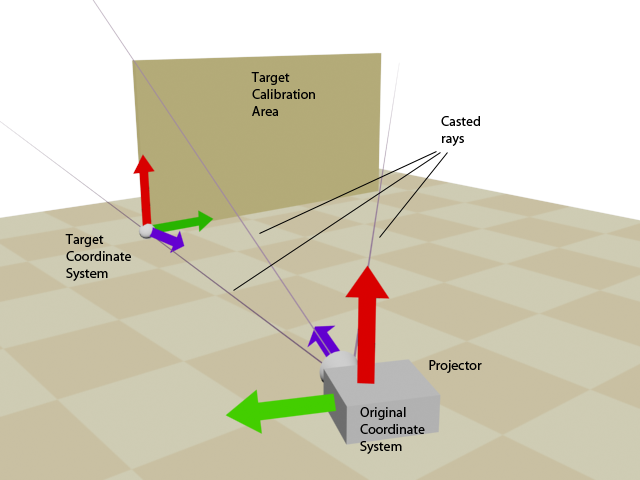
\includegraphics[width=0.7\textwidth]{./Cap2_videomapping/CalibrationSketch}
  \caption{Esquema de calibración.}
  \label{fig:CalibrationSketch}
\end{figure}
Usando las coordenadas en la pantalla de estos puntos y otros parámetros intrínsecos del proyector que son su resolución y el ángulo de proyección, es posible encontrar las coordenadas del punto con respecto al centro de proyección y por tanto la ecuación del rayo.
\[
a(t) = \vec{P} . t,	\mbox{ ecuación del rayo en dónde } \vec{P} \mbox{ es cualquier punto del rayo.}
\]
\[
\begin{cases}
P(X) = \frac{res_x}{2} - s_x \\
P(Y) = \frac{res_y}{2} - s_y \\
P(Z) = \frac{res_y}{2 \cdot \tan \frac{fov_y}{2}}
\end{cases}
\]
en donde $s_x$ y $s_y$ son las coordenadas del \emph{pixel}, $res_x$ y $res_y$ son la resolución horizontal y vertical del proyector y $fov_y$ es el ángulo de proyección vertical del proyector.

Aplicando esta ecuación a cada uno de los puntos a determinar se obtienen las ecuaciones paramétricas de los tres rayos. Vale aclarar que estos puntos $P$ son puntos de los rayos pero no necesariamente coinciden con los vértices de la superficie de calibración. Queda hallar las coordenadas de los vértices determinando el parámetro $t$ para cada ecuación. Para hallar este parámetro se resuelve un sistema de ecuaciones utilizando las tres ecuaciones de los rayos y las distancias conocidas entre estos puntos.
% Sistema de ecuaciones %
\[
\begin{cases}
\lVert{a(t_0) - b(t_1)} = j\rVert \\
\lVert{b(t_1) - c(t_2)} = k\rVert \\
\lVert{c(t_2) - a(t_0)} = l\rVert
\end{cases}
\]
siendo $a$, $b$ y $c$ los rayos y $j$, $k$ y $l$ las distancias entre las parejas de puntos.
La solución será entonces los parámetros $t_0$, $t_1$ y $t_2$ que satisfacen el sistema de ecuaciones no lineal.
Una aproximación a esta solución se puede obtener utilizando métodos numéricos, por ejemplo, el método \emph{trust-region-dogleg}\cite{TrustRegionDogleg}.
Una vez hallados los valores para $t_0$, $t_1$ y $t_2$, las coordenadas de los vértices de la superficie de calibración son $a(t_0)$, $b(t_1)$ y $c(t_2)$.
La base para el sistema de coordenadas con origen en el punto $P$ es:
\[
x' = \frac{b(t_1) - a(t_0)}{\lVert b(t_1) - a(t_0) \rVert},\quad y' = \frac{c(t_2) - a(t_0)}{\lVert c(t_2) - a(t_0)\rVert},\quad z' = -x' \times y'
\]
La ubicación del proyector en este nuevo sistema se obtiene proyectando cualquiera de los rayos en la nueva base de coordenadas.